%--------------------------------------------------------------------------------------
% Modelo de dissertação ou tese para o Instituto de Física da Universidade de São Paulo
% Autor: I. R. Pagnossin (irpagnossin at usp.br)
%--------------------------------------------------------------------------------------
\documentclass[
	a4paper,
	10pt,
	openany,
	oneside
	]{scrbook} % Classe do conjunto KOMA-Script

	\usepackage[utf8]{inputenc} % Codificação de entrada: UTF-8
	\usepackage[T1]{fontenc} % Codificação de saída: T1
	\usepackage{ae} % Fontes Computer Modern Roman vetoriais
	%\usepackage{mathptm} % Outra fonte que não as Computer Modern
	\usepackage[brazil]{babel} % Padrões de separação silábica e traduções do português
	\usepackage[colorlinks=true,linkcolor=red!50!black]{hyperref} % Hiper-texto (LaTeX -> PDF)
	\usepackage{xcolor}	% Cores
	\usepackage{makeidx} % Índice remissivo
	\usepackage{graphicx} % Inserção de figuras EPS, PDF, JPG ou PNG
	\usepackage{psfrag}	% Substituição de texto em figuras EPS
	\usepackage{indentfirst} % Endentação do primeiro parágrafo de cada seção
	\usepackage[squaren,binary]{SIunits} % Sistema internacional de unidades
	\usepackage[format=plain,margin=\parindent,font=small,labelfont=bf]{caption} % Legendas personalizadas
	\usepackage{subfigure} % Sub-figuras, e.g., fig.1(a), fig.3(c)
	\usepackage{quotchap} % Melhora o visual dos capítulos
	\usepackage{amsmath} % AMS-LaTeX
	\usepackage{icomma}	% Define a vírgula como separador de decimal
	\usepackage{colortbl}	% Cores em tabelas
	\usepackage[square,numbers]{natbib} % Citações personalizadas
	\usepackage{microtype} % Melhora a disposição das fontes
	\usepackage{tikz} % Utilizado para construir a capa
	\usepackage{booktabs} % Melhora a aparência de tabelas
	
	
	% Este pacote é utilizado para preencher as páginas deste modelo.
	% Substitua todas as ocorrências do comando \lipsum pelo seu texto.
	\usepackage{lipsum}

	% Espaço entre-linhas: 50% maior que o normal (p/ revisão).
	%\usepackage{setspace} % Revisão: veja o comando \setspace abaixo
	%\setstretch{1.5}

	% Cabeçalhos e rodapés personalizados
	\usepackage[ilines]{scrpage2}	
	\pagestyle{scrheadings}
	\chead{}
	\ohead{\headmark}	
	
	% Define onde procurar as figuras
	\graphicspath{{./arquivos/figuras/cap-introducao/}{./arquivos/figuras/cap-metodos/}}

	% Lista de exeções aos padrões de separação silábica.
	\hyphenation{}

	% Macros úteis.
	\newcommand{\cs}[1]{\texttt{\textbackslash\textcolor{blue!50!black}{#1}}} % Nome de comandos
	\newcommand{\pkg}[1]{\textsl{\textcolor{green!50!black}{#1}}} % Nome de pacotes
	\newcommand{\ctr}[1]{\textsf{\textcolor{orange!50!black}{#1}}} % Nome de contadores
	
	\newcommand\vetor[1]{\ensuremath{\boldsymbol{#1}}}
	\newcommand\foreign[1]{\textsl{#1}}	% Palavras estrangeiras	
	\newenvironment{dedicatoria}{\vspace*{\fill}\begin{flushright}}{\end{flushright}\pagebreak} % Dedicarória

	% Função sen (ao invés de sin, em inglês)
	\DeclareMathOperator{\sen}{sen}

%-------------------------------------------------------------------------------
\begin{document}

	%--------------------
	\frontmatter

	% Capa e ficha-catalográfica
	\newlength{\indentamount}
\setlength{\indentamount}{\parindent}

\newcommand{\nome}{de tal, Fulano}
\newcommand{\titulo}{Este é o título desta dissertação de mestrado ou tese de doutorado}
\newcommand{\cidade}{São Paulo}
\newcommand{\data}{\the\year}
\newcommand{\tipo}{Tese (Doutorado)}
%\newcommand{\tipo}{Dissertação (Mestrado)}
\newcommand{\universidade}{Universidade de São Paulo}
\newcommand{\instituto}{Instituto de Física}
\newcommand{\departamento}{O nome do departamento}
\newcommand{\orientador}{Prof. Dr. Beltrano Sicrano de tal}
\newcommand{\area}{Física}
\newcommand{\unitermos}{1. Fotodetectores; 2. Efeito Hall-quântico; 3. Física da Matéria Condensada}
\newcommand{\sbi}{USP/IF/SBI-016/2009}

%-------------------------------------------------------------------------------
% CAPA
%-------------------------------------------------------------------------------
\begin{titlepage}
	\begin{tikzpicture}[remember picture,overlay]
	
		% Universidade e instituto (cabeçalho)
		\node [yshift=-2cm] at (current page.north) {%
			\begin{minipage}{\textwidth}
				\centering
				\fontsize{15}{17}\usefont{T1}{pbk}{bx}{sc}
				\universidade\\\instituto
			\end{minipage}};
	
		% Título da tese/dissertação
		\node [yshift=+6cm] at (current page.center) {%
			\begin{minipage}{\textwidth}
				\centering\fontsize{20}{25}\usefont{T1}{pbk}{bx}{n}
				\titulo
			\end{minipage}
		};		
		
		% Autor da tese/dissertação
		\node [yshift=+1cm] at (current page.center) {%
			\begin{minipage}{\textwidth}
				\centering\fontsize{15}{17}\usefont{T1}{pbk}{bx}{n}
				O autor da tese/dissertação
			\end{minipage}
		};		
		
		% Orientador e banca examinadora
		\node [yshift=-4cm] at (current page.center) {%
			\begin{minipage}{\textwidth}
				\usefont{T1}{pbk}{m}{n}
				\textbf{Orientador:}\\
				\orientador\\[\baselineskip]
				\textbf{Banca examinadora:}\\
				Prof. Dr. Fulano de tal (USP)\\
				Prof\rlap.\textordfeminine Dr\rlap.\textordfeminine Sicrana de tal (USP)\\
				Prof. Dr. Beltrano de tal (USP) --- Presidente\\
				Prof\rlap.\textordfeminine Dr\rlap.\textordfeminine Beltrana de tal (USP)\\
				Prof\rlap.\textordfeminine Dr\rlap.\textordfeminine Fulana de tal (USP)
			\end{minipage}
		};
		
		% Descrição padronizada
		\node [yshift=-8cm,xshift=4cm] at (current page.center) {%
			\begin{minipage}{6cm}
				\rule[0ex]{\textwidth}{0.1pt}\par
				Tese de doutorado apresentada ao \instituto\ para a
				obtenção do título de Doutor em ciências.\par
				\rule[1ex]{\textwidth}{0.1pt}
			\end{minipage}};
				
		% Local e data (rodapé)
		\node [yshift=+2cm] at (current page.south) {%
			\begin{minipage}{\textwidth}
				\centering
				\usefont{T1}{pbk}{m}{n}
				\cidade\\\data
			\end{minipage}
		};
				
	\end{tikzpicture}
\end{titlepage}
%-------------------------------------------------------------------------------
% FICHA CATALOGRÁFICA
%-------------------------------------------------------------------------------
\newpage
\thispagestyle{empty}
\vspace*{\fill}
\begin{center}
	FICHA CATALOGRÁFICA\\
	Preparada pelo Serviço de Biblioteca e Informação\\
	do Instituto de Física da Universidade de São Paulo\par
	
	\medskip
	
	\fbox{\begin{minipage}{0.7\textwidth}
		\sloppy
		\setlength{\parindent}{\indentamount}
		\setlength{\parskip}{0.5\baselineskip}
		\nome\par
		\titulo\ --- \cidade, \data.\par
		\tipo\ --- \universidade.\par
		\instituto\ --- \departamento.\par
		\textbf{Orientador:} \orientador\par
		\textbf{Área de concentração:} \area\par
		\textbf{Unitermos:} \unitermos\par
		\medskip
		\noindent\sbi
	\end{minipage}}
\end{center}

	% Dedicatória
	\setcounter{page}{0}
	\newpage
	\begin{dedicatoria}
Dedico esta obra aos meus pais,\\
à minha esposa, aos meus filhos e\\
aos meus sobrinhos e sobrinhas
\end{dedicatoria}

	% Agradecimentos
	\newpage
	\section*{Agradecimentos}

\lipsum[1-5]

	% Resumo e abstract
	\newpage
	\addcontentsline{toc}{chapter}{Resumo/\foreign{Abstract}}
	\input{./arquivos/resumo}
	\section*{\foreign{Abstract}}
\lipsum[2]

	% Sumário
	\newpage
	\tableofcontents

	% Lista de figuras
	\newpage
	\addcontentsline{toc}{chapter}{\listfigurename}
	\setcounter{lofdepth}{2}
	\listoffigures
	
	% Lista de tabelas
	\newpage
	\addcontentsline{toc}{chapter}{\listtablename}
	\listoftables

	%--------------------
	\mainmatter
	\setheadsepline{0.2pt}

	% Capítulo: introdução
	\chapter{Introdução}
	\label{cap:introducao}
	\lipsum[1]\cite{Desrat:2006}

\section{Uma seção qualquer}

\lipsum[2-3]

\begin{figure}
	\centering
	\psfrag{S}[][]{Fonte}
	\psfrag{2}[][]{$2$}
	\psfrag{3}[][]{$3$}
	\psfrag{D}[][]{Dreno}
	\psfrag{5}[][]{$5$}
	\psfrag{6}[][]{$6$}
	\psfrag{1mm}[][]{\unit{1}{\milli\metre}}
	\psfrag{V1}[][]{$V_H$}
	\psfrag{V}[][]{$V$}
	\psfrag{I0}[][]{$I = 0$}
	\psfrag{I}[][]{$I$}
	\psfrag{RA}[][]{\shortstack{Região de\\ interesse}}
	\psfrag{200}[l][l]{\unit{200}{\micro\metre}}
	\psfrag{500}[l][l]{\unit{500}{\micro\metre}}
	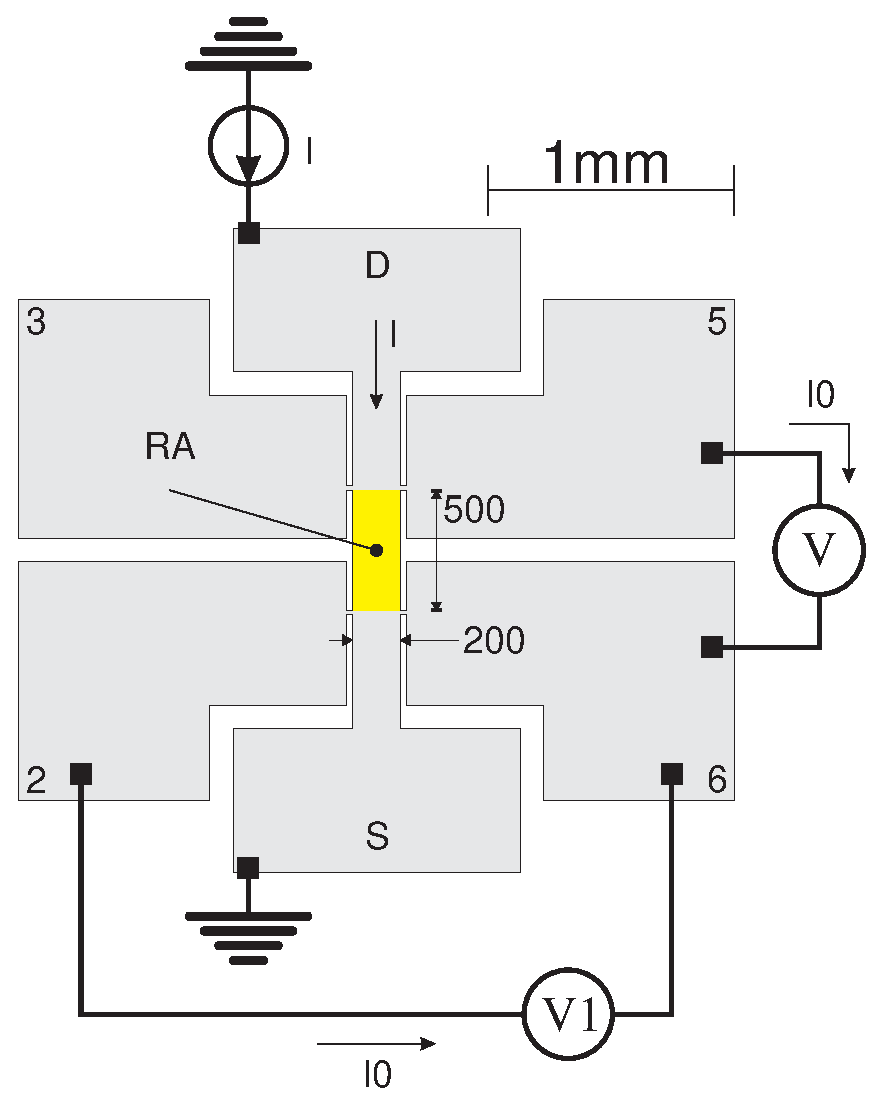
\includegraphics[height=0.4\textheight]{bH}
	\caption[Legenda curta]{o comando \cs{psfrag} (pacote \pkg{psfrag}) substitui os textos \emph{na figura EPS} por textos com a fonte deste documento. Mas isto só ocorre se a figura inserida aqui for EPS, ou seja, apenas se a compilação estiver produzindo um arquivo PostScript. Compare esta com a figura~\ref{fig:AB}, onde não efetuamos a substituição de texto.}
	\label{fig:if}
\end{figure}

\lipsum[4-5]

\section{Mais outra seção}

\lipsum[6]

Citando um livro: \cite{Eisberg:2000}

\lipsum[7-9]

	% Capítulo: conceitos e métodos
	\chapter{Conceitos e métodos}
	\label{cap:metodos}
	\lipsum[1]

Citando a figura do capítulo anterior: fig.~\ref{fig:if}

\section{Uma seção qualquer}

\lipsum[2-5]

	\begin{table}
		\centering
		\setlength{\belowcaptionskip}{0.5\baselineskip}
		\caption[Legenda curta]{tabelas são trabalhosas de se construir no \LaTeX, mas existem algumas ferramentas que podem ajudar. Por exemplo, o LaTable lhe permite criar tabelas visualmente e salvá-las no formato do \LaTeX. Além dele, alguns IDE (\foreign{Integrated Development Environment}) trazem consigo um \foreign{software} próprio para isso (o Kile é um exemplo). Finalmente, é possível baixar e instalar algumas macros para Excel e OpenOffice que convertem tabelas deles para o \LaTeX.}
		\label{tab:tabela}
		
		\begin{tabular}{ccc}
			\toprule
			Camadas	&	Espessuras (\nano\metre) & Observações\\
			\midrule
			GaAs & \multicolumn{2}{c}{Substrato semi-isolante (001)}\\
			\rowcolor{gray!20}GaAs & 50 & \foreign{Buffer} \\
			$[(\text{AlAs})_5(\text{GaAs})_{10}]\times10$	&	84 &	Super-rede (SR)	\\
			\rowcolor{gray!20}GaAs & 20 & \foreign{Buffer} \\
			\color{blue} GaAs:Si & $\sim\unit{1}{MC}$ & 	
				$n_\text{Si}=\unit{4}{\times\terad\centi\rpsquare\metre}$ \\ 
			\rowcolor{gray!20}\color{blue} GaAs & 30 & Barreira anterior\\ 
			\color{blue}$\text{In}_y\text{Ga}_{1-y}\text{As}$ & 10 & QW ($y = 16,53\%$) \\ 
			\rowcolor{gray!20}\color{blue} GaAs & 7 & Barreira posterior \\
			\color{blue} GaAs & 170 & \foreign{Buffer} \\ 
			\rowcolor{gray!20}GaAs:Si & 10 & $\unit{3,0\times10^{17}}{\centi\rpcubic\metre}$ \\
			\bottomrule
		\end{tabular}
	\end{table}

\section{Mais outra seção}

\lipsum[6]

\begin{equation}\label{eq:pitagoras}
\sen^2\phi + \cos^2\phi = 1.
\end{equation}

\lipsum[7-9]

	%--------------------
	\appendix

	\chapter{Lista de símbolos}
	\label{ap:simbolos}
	\lipsum[1]

\section{Uma seção do apêndice}

\lipsum[2]

	\begin{figure}
		\centering
		
		\null\hfill
		\subfigure[Legenda curta][Legenda dessa figura]{
			\label{fig:figA}
			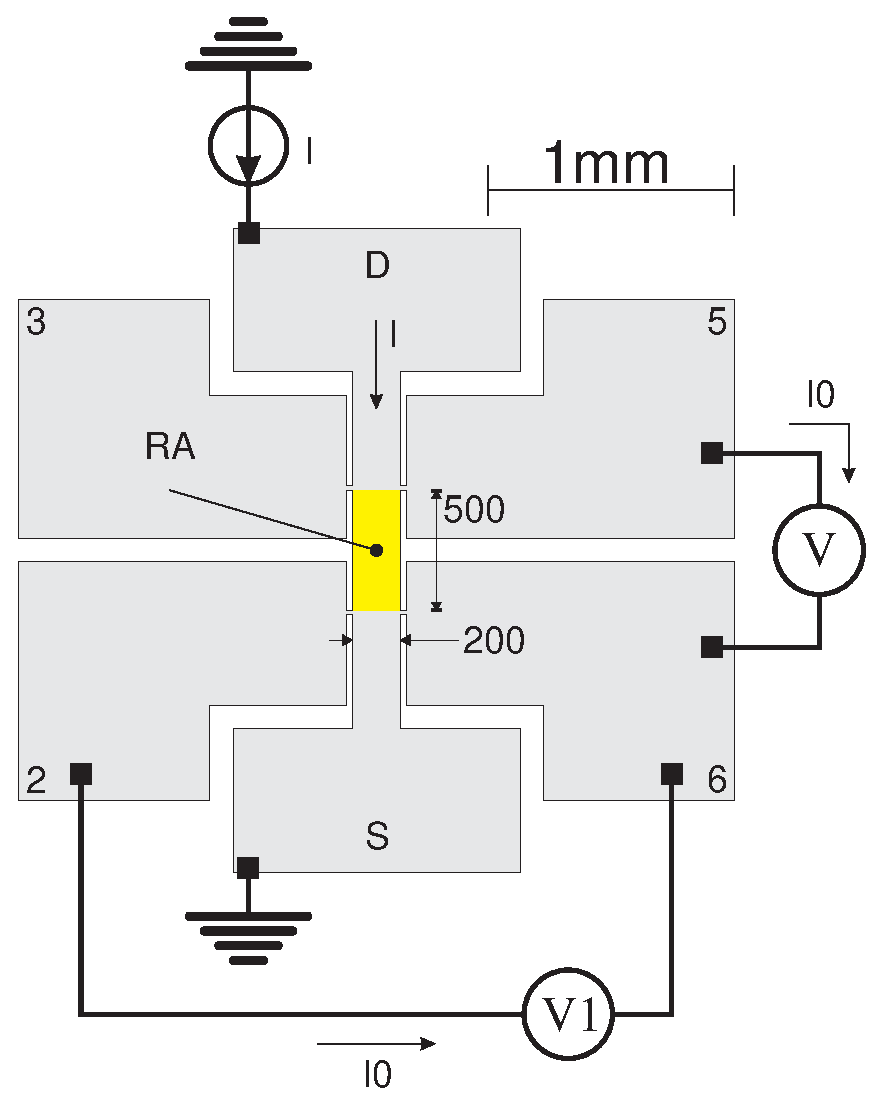
\includegraphics[width=0.4\textwidth]{bH}}%
		\hfill
		\subfigure[Legenda curta][Legenda dessa figura]{
			\label{fig:figB}
			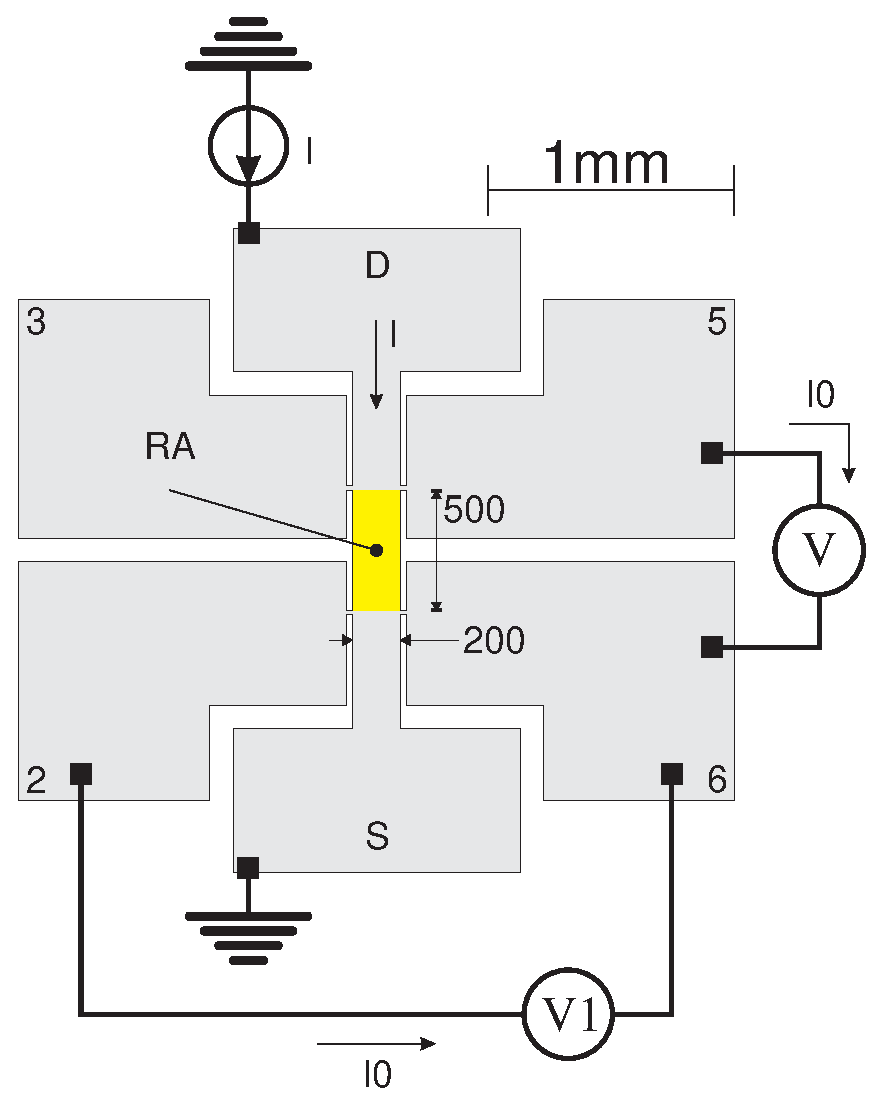
\includegraphics[width=0.4\textwidth]{bH}}%
		\hfill\null
		
		\caption[Legenda curta]{Legenda comum às duas figuras. A versão curta das legendas das duas figuras acima só aparecerão na lista de figuras se você definir o contador \ctr{lofdepth} (profundidade da lista de figuras) igual a 2.}
		\label{fig:AB}
	\end{figure}
	
\lipsum[6-7]

	% Bibliografia
	\newpage
	\addcontentsline{toc}{chapter}{\bibname}
	\bibliographystyle{./arquivos/Science}
	\bibliography{./arquivos/referencias}

\end{document}
%-------------------------------------------------------------------------------